\subsubsection*{a) Choice of Stores}
\medskip
For this analysis, we have selected two stores. The first store will be \emph{Main Street A}, as this store is located in a high-traffic shopping area with an established demand affected by seasonal variation and was established before COVID and has survived COVID. 

The second store that has been selected is \emph{Station B}. Since this is a newer location near a transport hub, it shows more irregular and yet high demand levels and has a right-skewed distribution.

Because \emph{Main Street B} is relatively stable, has a lower average demand and has fewer distinguishing characteristics, it would not add any analytical contrast to the two selected stores.

In addition, \emph{Station A} is also located in a high traffic zone. The store presents a more complex multi-modal distribution and has a higher day-to-day variability, which may make it less relevant for reliable parametric modeling. 

By selecting \emph{Main Street A} and \emph{Station B}, we capture the contrast between a steady, well-understood location and a newer, high-variance location, which allows us to demonstrate how different distributional assumptions apply across different demand contexts.

\subsubsection*{b) Specification of Demand Distributions}
\medskip

To specify the demand distributions, we look back at the results from task 5, since that is where we analyzed the shape of the demand using histograms, box plots, and time series visualizations from all stores. 

For \emph{Main Street A}, the histogram looked like a bimodal distribution, probably driven by the differing behavior of the customers between weekdays and weekends. However, when the data are filtered by individual weekdays, the demand appears to be approximately normally distributed. Hence, the use of a \textbf{normal distribution} as a reasonable parametric approximation is logic for short-term forecasting, especially when adjusting for the day of the week. 
This choice is further supported by \cite{ramaekers2008}, who write in their paper that when the mean demand is relatively high compared to its variance, as in the case for Main Street A, the normal distribution can serve as a suitable approximation in inventory models. For example, on Fridays, the demand at the store \emph{Main Street A} shows a high concentration around the center and relatively low skewness, which aligns well with the conditions under which a normal model performs consistently.

For \emph{Station B}, Task 5 shows a right-skewed distribution with a high concentration of average demand days and some rare sharp peaks. This pattern can be seen in the histogram, as well as in the box plot and time series plot. Based on this, we choose a \textbf{log-normal} distribution to capture the positive skewness and the scaling effect of high-demand conditions. The log-normal model is particularly suitable for nonnegative, right-skewed shopping demand (\cite{rojas2021}).


\subsubsection*{c \& d) Point Estimates and Intervals for the Theoretically Optimal Quantities}
\medskip

In this section, we estimate the optimal order quantities $Q^*$ for the short term, by using the Normal and Log-Normal parametric approach. These estimates are based on the critical fractile formula, which has been derived in section 2. These incorporate adjusted cost values $\tilde{c}$ that incorporate the clearance price and the shipping costs.

The following table summarizes the point estimates and the 95\% confidence intervals for the \emph{Main Street A} store for the different weekdays.

\begin{figure}[H]
    \centering
    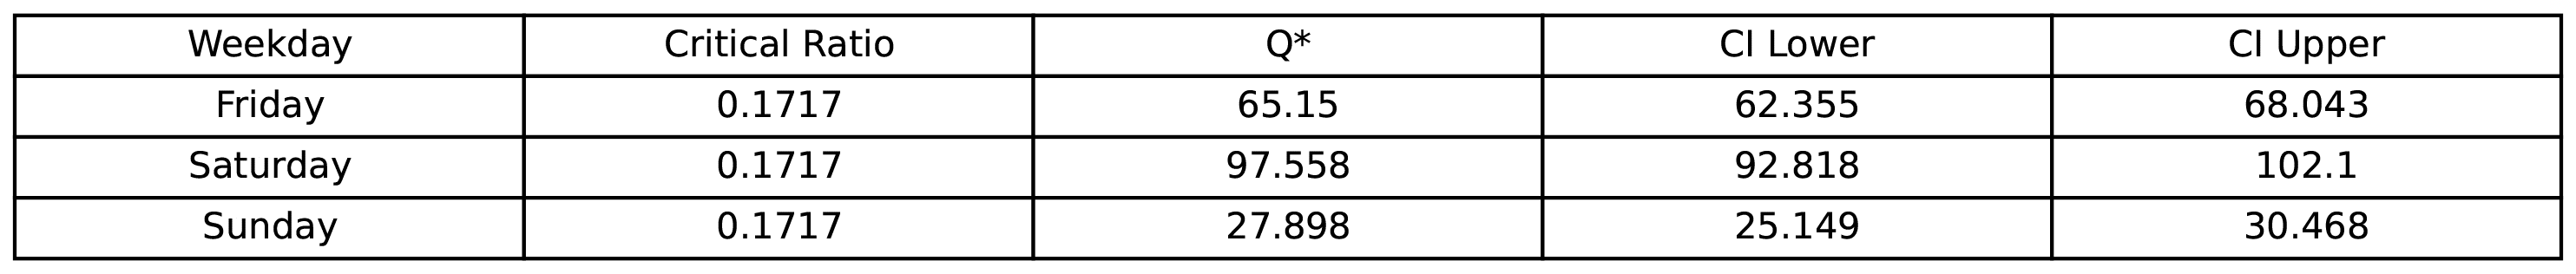
\includegraphics[width=1\textwidth]
    {figures/Figure_Normal_MainStreetA.png}
    \caption{Table of point estimates and confidence intervals for Main Street A with normal distribution}
    \label{fig:Table for Main Street A}
\end{figure}

For Main Street A, the demand is more predictable and increases on weekends, with its peak on Saturday at 97.56 units, while remaining mild on Friday, with 65.15 units, and quite lower on Sunday, with 27.90 units. The tighter confidence intervals reflect consistent and well-distributed foot traffic. This pattern is typical for stores located in shopping districts, where the demand tends to be more stable and evenly distributed throughout the day and week due to flexible and recreational shopping behavior (\cite{berry2016}).

Next, in the following table, the point estimates and the 95\% confidence intervals for the \emph{Station B} store are shown for different weekdays.

\begin{figure}[H]
    \centering
    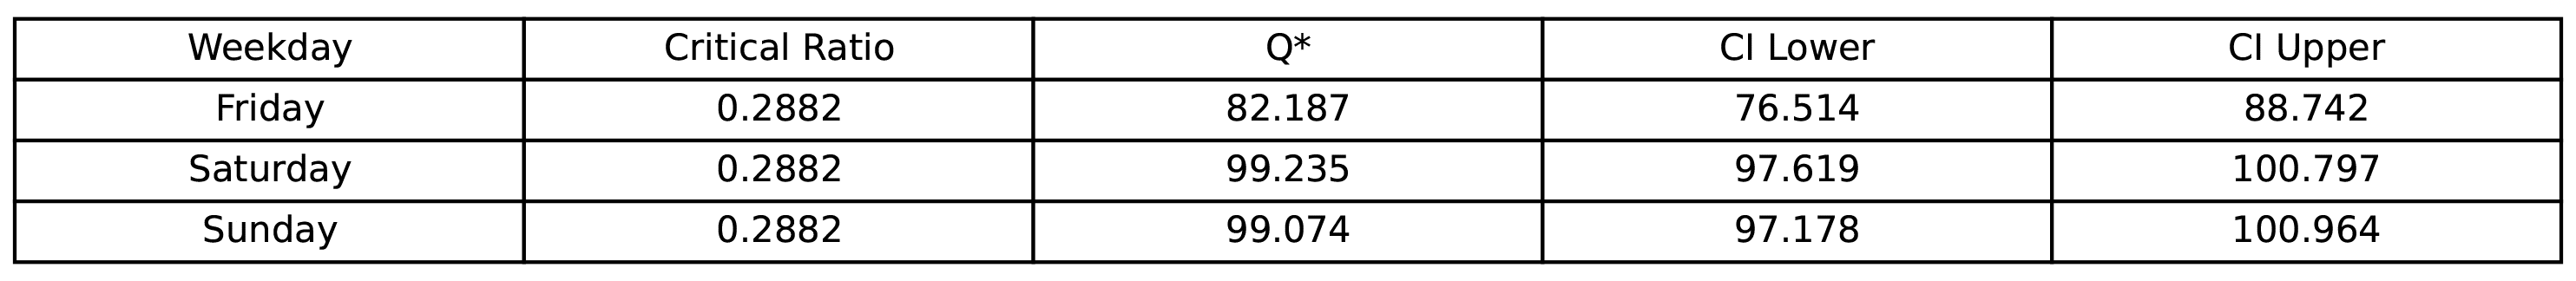
\includegraphics[width=1\textwidth]
    {figures/Figure_LogNormal_StationB.png}
    \caption{Table of point estimates and confidence intervals for Station B with lognormal distribution}
    \label{fig:Table for Station B}
\end{figure}

In contrast, Station B shows a higher and more volatile demand, with estimates almost being equal on the weekends and on Friday a little lower with 82.19 units. The narrow confidence intervals on weekends indicate a concentrated but predictable peak behavior. These patterns are in line with the findings of Berry et al. (2016), who note that shops near transport hubs experience highly time-specific demand peaks driven by transit flows, leading to a right-skewed and more variable demand distribution.
In general, the variation in the choice of the distributions and the resulting estimates is based on the spatial context of each store. This confirms that inventory strategies must be different for each location and driven by data.